\documentclass[
11pt,%
tightenlines,%
twoside,%
onecolumn,%
nofloats,%
nobibnotes,%
nofootinbib,%
superscriptaddress,%
noshowpacs,%
centertags]%
{revtex4}
\usepackage{ljm}
\usepackage{listings}

\lstset{
language=C++,
basewidth=0.5em,
xleftmargin=45pt,
xrightmargin=45pt,
basicstyle=\small\ttfamily,
keywordstyle=\bfseries\underbar,
numbers=left,
numberstyle=\tiny,
stepnumber=1,
numbersep=10pt,
showspaces=false,
showstringspaces=false,
showtabs=false,
frame=trBL,
tabsize=2,
captionpos=t,
breaklines=true,
breakatwhitespace=false,
escapeinside={\%*}{*)}
}

\begin{document}

\titlerunning{Process Mining}
\authorrunning{Savin et al.}

\title{Process Mining: Realization and Optimization of Process Discovery Algorithm}

\author{\firstname{G.~I.}~\surname{Savin}}
\email[E-mail: ]{savin@jscc.ru}
\affiliation{Joint Supercomputer Center of the Russian Academy of Sciences -- branch of Scientific Research Institute of System Analysis of the Russian Academy of Sciences, Leninsky prospect 32a, Moscow, 119334, Russia}

\author{\firstname{A.~D.}~\surname{Chopornyak}}
\email[E-mail: ]{chopor@jscc.ru}
\affiliation{Joint Supercomputer Center of the Russian Academy of Sciences -- branch of Scientific Research Institute of System Analysis of the Russian Academy of Sciences, Leninsky prospect 32a, Moscow, 119334, Russia}

\author{\firstname{A.~A.}~\surname{Rybakov}}
\email[E-mail: ]{rybakov.aax@gmail.com}
\affiliation{Joint Supercomputer Center of the Russian Academy of Sciences -- branch of Scientific Research Institute of System Analysis of the Russian Academy of Sciences, Leninsky prospect 32a, Moscow, 119334, Russia}

\author{\firstname{S.~S.}~\surname{Shumilin}}
\email[E-mail: ]{shumilin@jscc.com}
\affiliation{Joint Supercomputer Center of the Russian Academy of Sciences -- branch of Scientific Research Institute of System Analysis of the Russian Academy of Sciences, Leninsky prospect 32a, Moscow, 119334, Russia}

\firstcollaboration{(Submitted by S.~S.~Submitter)}

\received{May 01, 2020}

\begin{abstract}
Abstract.
\end{abstract}

\subclass{68R10} % Enter 2010 Mathematics Subject Classification.

\keywords{Process mining, process discovery algorithm, Petri nets, process model, event logs.}

\maketitle

\section{Introduction}

Process mining is a collection of approaches and methods for extracting process related information from event logs.
Process mining is closely related to areas such as business process management (BPM) and workflow management (WFM).
WFM technology has historically been primarily aimed at automating business processes from a mechanical point of view, while using BPM approaches, special attention is paid to other aspects in which bottlenecks can be hidden (human factor, organization features, fuzzy rules, and others).
Currently, many process-aware information systems (PAIS), in addition to the classic WFM tools, include BPM extensions and process mining approaches.
However, often these systems remain analysis and notification systems, being insufficiently integrated into the digital space.
Along with the term PAIS, the term BPMS (BPM system) or simply PMS (process management system) is also used for such systems.

Any process analysis system works with a process model that is written using one or more notations.
These notations represent the essence of the process and are essentially macro-descriptions of oriented graphs of a special kind.
The main objects of process models are activities, states, transitions and subprocesses.
Transitions between different activities are also called dependencies.
The set of dependencies between activities and also additional conditions imposed on the process model give rise to many possible sequences of state changes, or many scenarios of the process.
Depending on the details of the processes, additional attributes of any objects of the process model can be used: time references, duration of activities, dependency logic, resources and strategies for their use, roles of activity performers, and many others.
Such a variety that arises in the modeling of processes generates a huge number of methods for analyzing processes and scenarios, and can serve as a source of useful and not always obvious knowledge used to optimize processes.

Process models recorded using formal notation can be used for various purposes: a review from various points of view, discussion of a process model between all participants, preparation of documentation (including in automatic mode), verification (some obvious errors may be detected just by analyzing the topology of the model graph, for example, it can be dead sections of the process, deadlocks, infinite loops and others), performance analysis (using simulations on the process model can be bottlenecks identified and eliminated), visualization of the process to simplify the analysis, specification (from the formal model, descriptions of interfaces and interaction protocols can be generated even before integration into a single digital space), configuration (the description of the process model can be used to configure the system when its implementation).
Typically, when developing a process, there is both an informal model (used for discussion and documentation) and a formal model suitable for simulations (used for analysis and improvement). 

Informal models are often divorced from life, abstract, idealized, while formal models, on the contrary, are too detailed and often understandable only to the actual developers of the model.
There is no middle ground between these two models, and this often leads to additional risks when developing a process model, since in fact the tested and analyzed executable model is very different from the model at the presentations.
But even this is not the main problem.

The main problem of any process model is that it is not known in advance how much the model relates to reality.
In reality, people are included in the processes, the logic of their interaction with the system is immeasurably complex, and accurate modeling of a person’s behavior, his motivation system and other features is impossible in a fixed process model (the process model cannot be rebuild taking into account each individual person).
As a result, it may turn out that a superbly worked out and debugged process model is not viable when implemented in a working system.
The only way out of this situation can be the presence of feedback between the process taking place in the real world and the process model.
Such feedback in terms of the process mining approach is expressed in the registration of events about individual activities and the recording of event data in special repositories called event logs.

Event logs are filled in during the operation and monitoring of a working system and should be used to optimize the process model when re-designing this model.
However, at present, the data accumulated during monitoring the functioning of the system are not fully used to analyze the performance of the process model.
Very few organizations verify compliance of accumulated data and the process model, and often the reasons for re-designing the process model are not performance issues, but external factors, such as changes in legislation, policies, standards, or changes in external cooperation.
Thus, there are risks that the process model may be repeatedly redesigned, but retain the weaknesses and bottlenecks that lead to constant low system performance.
There is a kind of vicious circle, the only way out of which is the intellectual analysis of monitoring data (event logs), with subsequent feedback when improving the process model.

Process mining is a new discipline, with the help of which the analysis of the monitoring data of a working system is carried out, on the basis of which you can get knowledge about the actual course of a process, which allows you to work with the process itself, and not with its idealized model.

While applying process mining technology, the business process model interacts with a working information system, the outside world and accumulated data.
The process model is transformed into a process implemented within the information system through which interaction with the outside world is carried out.
At the same time, events coming from the outside world through an information system are recorded in event logs.
The main application of process mining arises when analyzing the interaction of a process model and accumulated data.

There are three main areas of process mining.
The first direction is the construction of a process model based on accumulated data (process discovery).
It consists in the analysis of the actual accumulated data on the course of the real process (fixed chains of data flows, a log of the interaction of process participants with each other, message passing between process participants) and the construction of a process model based on it without using information about the designed idealized model.
The second area is called conformance testing.
The purpose of this type of analysis is to verify the conformity of the developed model and the event logs related to this model.
When conducting this check, it is possible to detect regions in the process model that are not sufficiently covered by data from event logs or regions with insufficiently clear logic, within which the course of the real process slows down due to the additional costs of overcoming these difficulties.
For example, in the place of a fuzzy description of the logic of the process, additional coordination of some action that is not reflected in the process model may be required.
In this case, the model can demonstrate high performance, however, with real flow, the process will slow down or even block.
The third area or process mining is process improvement based on analysis (process enhancement).
If checking the conformity of the process model and its data helps to find places where the process model diverges from reality, then in this direction it is possible to develop recommendations on how to change the process model in order to reduce this discrepancy.
Improvements may relate to the modification of the process model to more accurately reflect reality, and may cause the model to expand if the logic of the existing model is too meager to reflect the complex interactions of the process participants.

It is worth noting that the logic of the process, data flows, interaction within the process, messaging are the most simple aspects that affect process mining.
However, technology is not limited to these aspects.
Resource allocation, planning issues, decision rules, complex interaction logic, probabilistic events all of these aspects also apply to process mining and can be analyzed using the tools of this technology.

This article discusses an algorithm for constructing a real process based on data from an event log and discusses ways to optimize this algorithm.

\section{Simple Process Discovery Algorithm}

In this article we will consider the description of the process model using workflow nets (WFN).
WFN reflects only the sequence of activities during the flow of the process scenario and does not affect other aspects of the analysis.
WFN is a directed graph whose edges are capable of transmitting tokens that reflect the course of the scenario.

There are two types of WFN nodes.
The nodes of the first type are tokens places (on the diagrams of process models are shown below with white rectangles, place labels are denoted $p0$, $p1$, etc.).
The nodes of the second type represent the activity of the process (in the diagrams of the process models are shown below with black rectangles, the activity labels are named $a$, $b$, etc.).
Two places are specially allocated in WFN: $I$ is the global input from which the scenario starts, $O$ is the global output where the scenario ends (these special places are shown by gray rectangles on the diagrams of process models).

WFN edges can connect only nodes of different types (that is, only activity can be a predecessor or successor of a place, only a place can be a predecessor or successor of an activity).
During the course of the process, some activity can be performed only if all the predecessor token places of this node contain tokens.
After performing some activity in WFN, tokens from the predecessor nodes are deleted, after which new tokens are created, which are distributed along all output edges and are placed in all successor nodes of this activity.

\begin{figure}[h]
\setcaptionmargin{5mm}
\onelinecaptionsfalse % if the caption is multiline
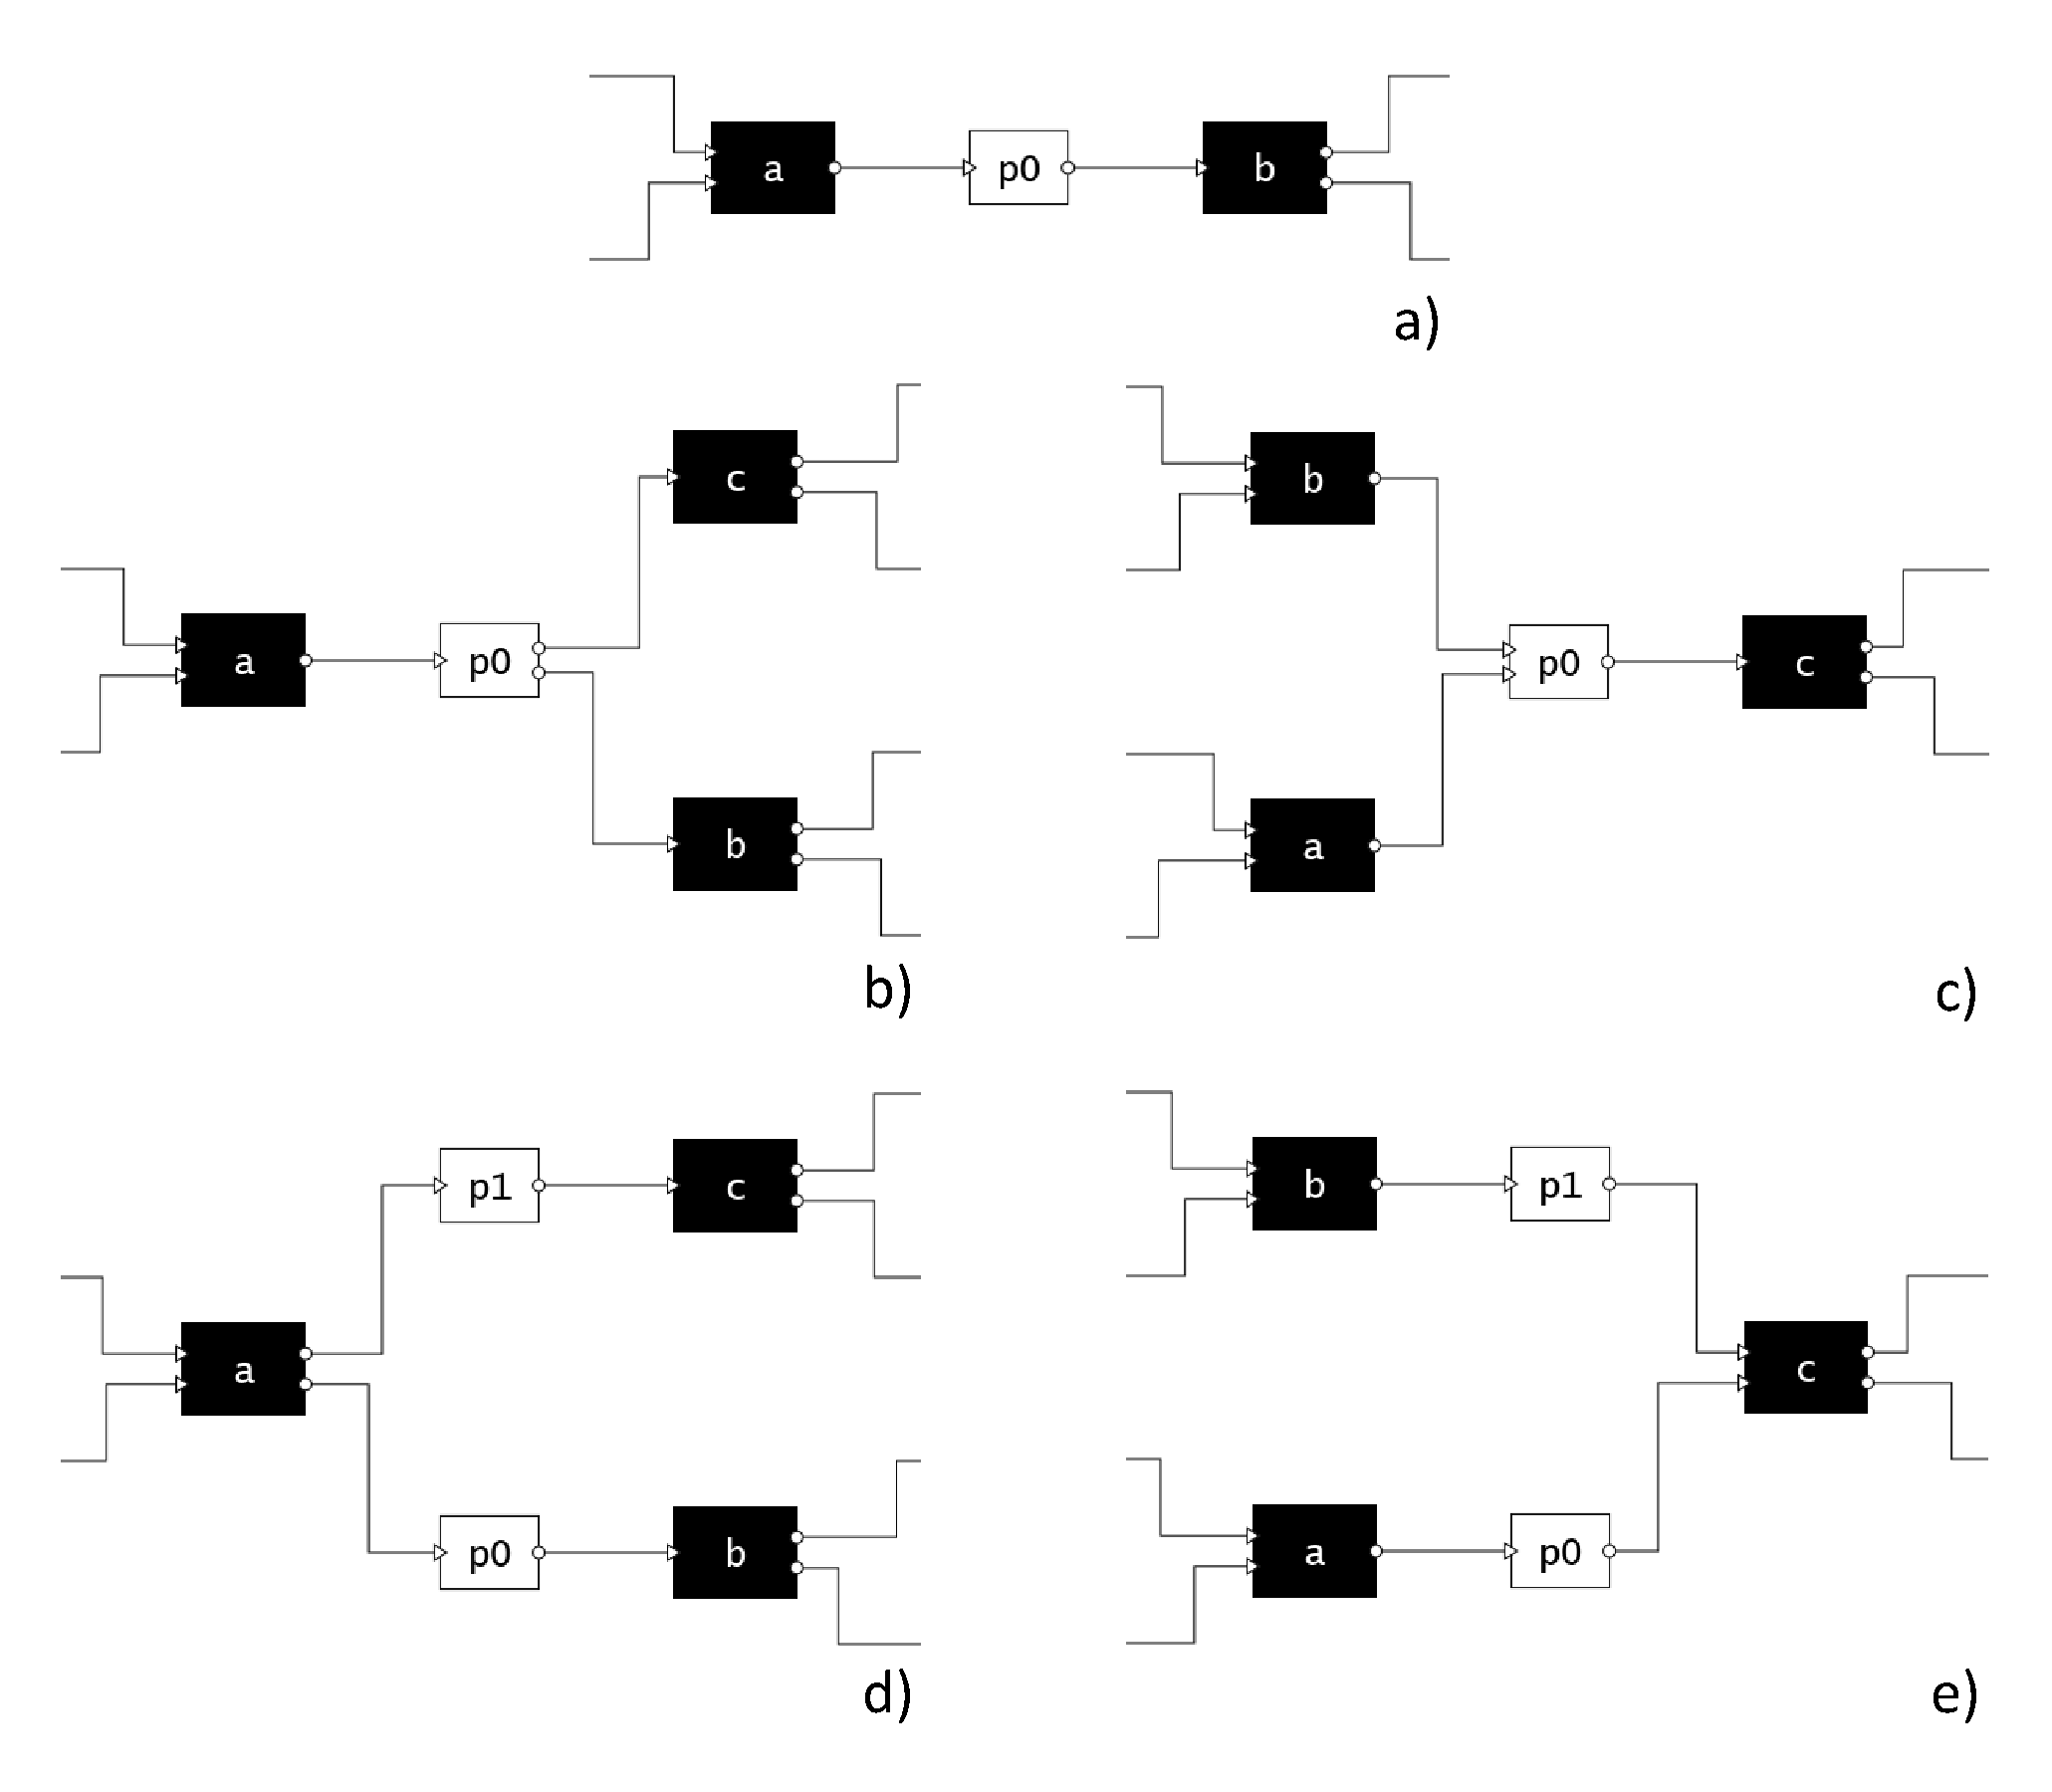
\includegraphics[width=0.8\textwidth]{pics/wfn-patterns.pdf}
\captionstyle{normal}\caption{Process patterns in WFN model. a) Sequence, b) XOR-split, c) XOR-join,\\d) AND-split, e) AND-join.}
\label{fig:wfn-patterns}
\end{figure}

Consider the main local patterns of the process that can be displayed using WFN (Figure~\ref{fig:wfn-patterns}).

Figure~\ref{fig:wfn-patterns} a) shows the usual sequence of activities $a \rightarrow b$.
This template prescribes that after the $a$ activity is completed, the token will be placed in the place of $p0$.
After that, it turns out that the condition $b$ is fulfilled that all its predecessors contain tokens (since the only predecessor $b$ is $p0$).
Thus, the $b$ activity will be performed, the token will be removed from the place $p0$, and new tokens will be sent along the output edges to the nodes-successors of the $b$ activity.
     
Figure~\ref{fig:wfn-patterns} b) shows an XOR-split template that implements the selection of one of the activities after the execution of the $a$ activity.
After the activity $a$ has been completed, the place $p0$ is occupied by a token, which can be used when only one of the activities $b$ or $c$ is performed.
Thus, it is possible to execute either a sequence of activities $a \rightarrow b$ or a sequence $a \rightarrow c$.

The figure~\ref{fig:wfn-patterns} c) shows the XOR-join template, which by analogy implements either a sequence of activities $a \rightarrow c$ or a sequence of activities $b \rightarrow c$.

The figure~\ref{fig:wfn-patterns} d) shows the AND-split pattern, which implements the execution of both $b$ and $c$ after the $a$ activity.
As soon as the $a$ activity is completed, tokens fall into the places $p0$ and $p1$, which make it possible to execute the $b$ and $c$ activities.
In this case, the order in which these activities will be performed is not important.

The figure~\ref{fig:wfn-patterns} e) shows the AND-join pattern, demonstrating that the activity $c$ can be performed only after the execution of both activities $a$ and $b$.
The $c$ activity requires for its execution the presence of tokens immediately in $p0$ and $p1$, and this can happen only after the execution of both $a$ and $b$ activities.
The execution order of the $a$ and $b$ activities is not important in this case.

After describing this simplified process model using WFN, we can proceed directly to the algorithm for constructing the model based on the event log.
In this case, an event log is simply a list of scenarios, each of which is an ordered sequence of activities.
According to the provided event log, it is required to build a process model described using WFN that implements all the scenarios from this log.

We will consider simple scenarios in which it will be seen how strongly the event log entries affect the real process model.
For example, let us have an ideal model of a process, which consists of a fixed sequence of activities that must be performed in a strictly defined sequence.
Here is the sequence of activities: $a \rightarrow b \rightarrow c \rightarrow d \rightarrow e \rightarrow f$.
This sequence of activities corresponds to the following process model shown in the figure~\ref{fig:origin1}.

\begin{figure}[h]
\setcaptionmargin{5mm}
%\onelinecaptionsfalse % if the caption is multiline
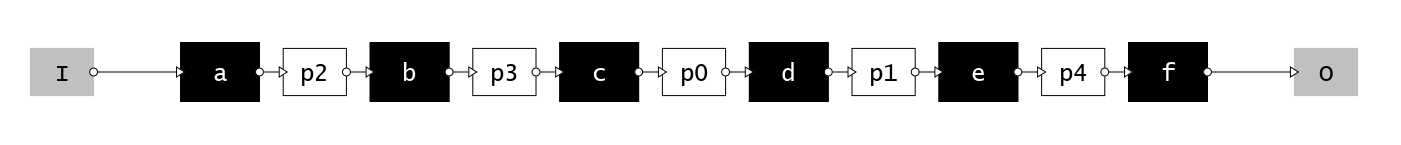
\includegraphics[width=0.95\textwidth]{pics/origin1.png}
\captionstyle{normal}\caption{Process model that build from one scenario $a \rightarrow b \rightarrow c \rightarrow d \rightarrow e \rightarrow f$.}
\label{fig:origin1}
\end{figure}

Even if all participants in the process agree with such a specific sequence of activities that is necessary for the scenario to proceed, then in reality situations usually happen when the process proceeds differently.
Imagine a simple situation when, due to rush or force majeure, all intermediate activities in the scenario execution were omitted and the entry $a \rightarrow f$ appeared in the event log.
Figure~\ref{fig:second1} shows a new process model that also reflects this simplified scenario.

\begin{figure}[h]
\setcaptionmargin{5mm}
%\onelinecaptionsfalse % if the caption is multiline
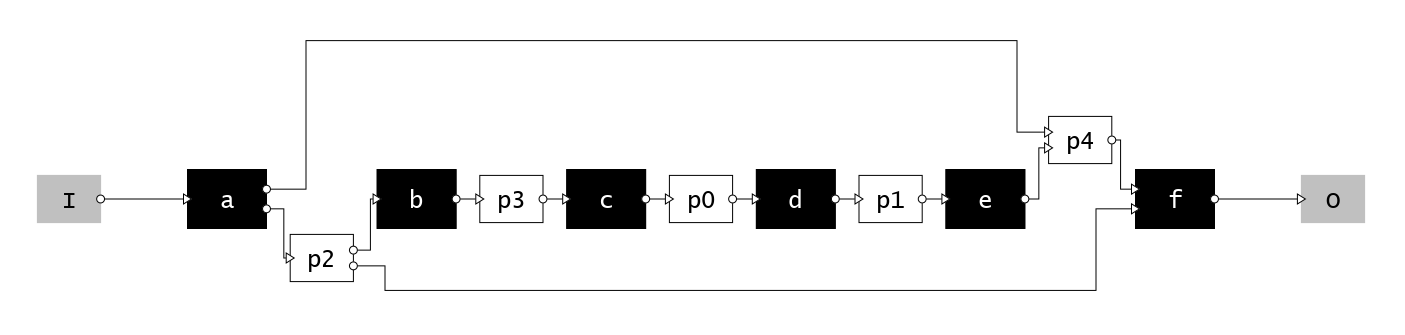
\includegraphics[width=0.95\textwidth]{pics/second1.png}
\captionstyle{normal}\caption{Adjusted process model after processing the scenario $a \rightarrow f$.}
\label{fig:second1}
\end{figure}

In this figure, we already see the emergence of the XOR-split and XOR-join patterns, and in general the process model has become much more complicated.

And now let's look at an even more extended event log, in which there are scenarios with other deviations.
In particular, we consider a scenario with a violation of the order of activities, a partial scenario, and a scenario with the repeated execution of certain sequences of activities.
Let's collect the full event log, it will look like this:

\begin{eqnarray*}
a \rightarrow b \rightarrow c \rightarrow d \rightarrow e \rightarrow f \\
a \rightarrow f \\
a \rightarrow b \rightarrow d \rightarrow c \rightarrow e \rightarrow f \\
a \rightarrow b \rightarrow c \\
a \rightarrow b \rightarrow c \rightarrow d \rightarrow e \rightarrow b \rightarrow c \rightarrow d \rightarrow e \rightarrow f
\end{eqnarray*}

When building a process model from the presented event log, we get the circuit shown in the figure~\ref{fig:third1}.

\begin{figure}[h]
\setcaptionmargin{5mm}
%\onelinecaptionsfalse % if the caption is multiline
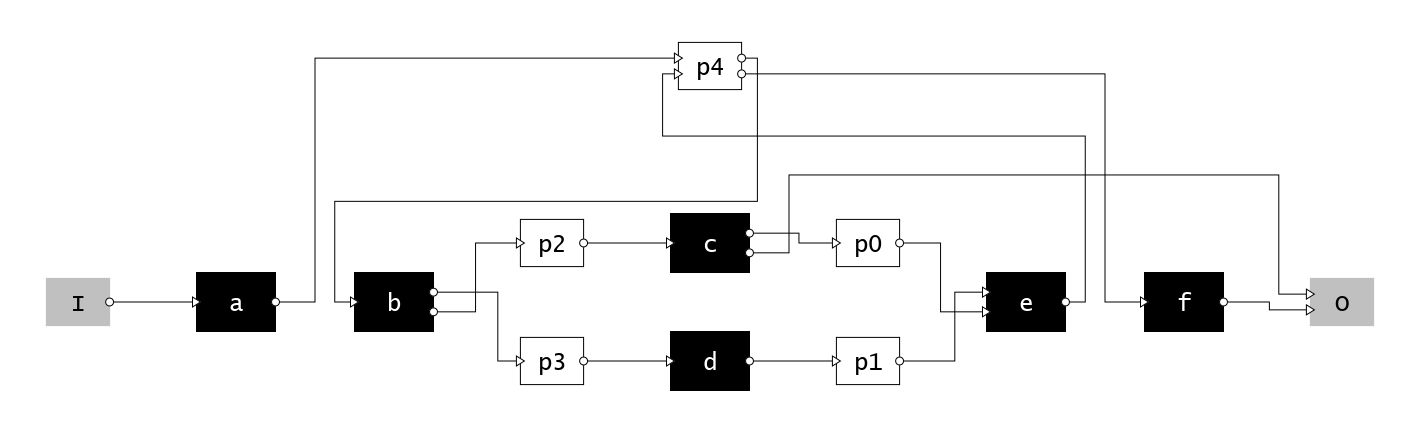
\includegraphics[width=0.95\textwidth]{pics/third1.png}
\captionstyle{normal}\caption{A process model based on an event log containing distorted scenarios.}
\label{fig:third1}
\end{figure}

This model of the process, of course, does not look like the ideal model from the figure~\ref{fig:origin1}.
It is also obvious that any analysis should be carried out using this real model, and not an ideal one.
The construction of a real model from the event log can only be performed automatically, since any distortion of real scenarios significantly affects the topology of the model.
We also note that the above examples show completely trivial scenarios that do not come close to the complexities of real-life business processes.
Therefore, to build models of real processes for real event logs, efficient algorithms are required.

Let us describe the simplest algorithm for constructing a process model from an event log.
In the process of describing the algorithm, we will immediately show its results on the already considered model event log (we denote it by $L$).

So we have an event log

\begin{equation}
\begin{aligned}
L = [
&{a \rightarrow b \rightarrow c \rightarrow d \rightarrow e \rightarrow f},\\
&{a \rightarrow f},\\
&{a \rightarrow b \rightarrow d \rightarrow c \rightarrow e \rightarrow f},\\
&{a \rightarrow b \rightarrow c},\\
&{a \rightarrow b \rightarrow c \rightarrow d \rightarrow e \rightarrow b \rightarrow c \rightarrow d \rightarrow e \rightarrow f}
]
\end{aligned}
\end{equation}

First, we need to determine the set of all activities present in the event log (we denote it $A$).
In addition, we need to define the set of activities with which the scenarios from the event log start ($A_I \subset A$), as well as the activities that end the scenarios from the event log ($A_O \subset A$).

\begin{equation}
\begin{aligned}
&A = \{a, b, c, d, e, f\} \\
&A_I = \{a\} \\
&A_O = \{c, f\}
\end{aligned}
\end{equation}

The next step requires the construction of a matrix of activity sequences ($M_S$).
This matrix is square; it has size $| A | \ times | A |$, and its element $M_S[x, y]$ contains 1 if there is a scenario in the event log that contains the sequence $x \ rightarrow y$.

The $M_S$ matrix for our test event log is as follows:

\begin{equation}
M_S = \begin{vmatrix}
\ & [a] & [b] & [c] & [d] & [e] & [f] \\
[a] & 0 & 1 & 0 & 0 & 0 & 1 \\ 
[b] & 0 & 0 & 1 & 1 & 0 & 0 \\
[c] & 0 & 0 & 0 & 1 & 1 & 0 \\
[d] & 0 & 0 & 1 & 0 & 1 & 0 \\
[e] & 0 & 1 & 0 & 0 & 0 & 1 \\
[f] & 0 & 0 & 0 & 0 & 0 & 0
\end{vmatrix}
\end{equation}

Next, the relationship matrix $M_R$ is constructed.
It has the same size as the $M_S$ matrix, and its elements determine the relationships between activities that should be reflected in the constructed process model.
The strict follow relationship between the $x$ and $y$ activities (we will denote it by $x \Rightarrow y$) means that in the event log there is a scenario in which $x \rightarrow y$, but there is no such scenario in which $y \rightarrow x$.
In other words, the $x$ and $y$ activities are related by a strict follow relationship if $M_S[x, y](1 - M_S[y, x]) = 1$.
Similarly, the activities of $x$ and $y$ can be called parallel, if in some scenarios $x$ may follow $y$, and in other scenarios $y$ may follow $x$.
The condition for parallel activities is $M_S[x, y]M_S[y, x] = 1$ (designation $x \ || \ y$).
If, in no scenarios, the sequences $x \rightarrow y$ or $y \rightarrow x$ are detected, then the relation between such activities will be called uncertainty.
The uncertainty condition is $(1 - M_S[x, y])(1 - M_S[y, x]) = 1$ (designation $x \ ? \ y$).

For the considered event log, the $M_R$ matrix is as follows:

\begin{equation}\label{eqn:r}
M_R = \begin{vmatrix}
\ & [a] & [b] & [c] & [d] & [e] & [f] \\
[a] & ? & \Rightarrow & ? & ? & ? & \Rightarrow \\ 
[b] & \Leftarrow & ? & \Rightarrow & \Rightarrow & \Leftarrow & ? \\
[c] & ? & \Leftarrow & ? & || & \Rightarrow & ? \\
[d] & ? & \Leftarrow & || & ? & \Rightarrow & ? \\
[e] & ? & \Rightarrow & \Leftarrow & \Leftarrow & ? & \Rightarrow \\
[f] & \Leftarrow & ? & ? & ? & \Leftarrow & ?
\end{vmatrix}
\end{equation}

After constructing a matrix of relations between activities, we can proceed to constructing set of token places in the process model ($P$).
A token place must be built for each such pair of disjoint subsets of activities $X \subset A$, $Y \subset A$, which satisfies two conditions.
Firstly, any two activities from $X$ are related by the uncertainty relation, also any two activities from $Y$ are connected by the uncertainty relation.
Secondly, any activity $x \in X$ is associated with any activity $y \in Y$ by the ratio $x \Rightarrow y$.
In this case, the token place $p(X, Y)$ is built, all the activities from $X$ become its predecessor nodes, and all activities from $Y$ become the successor nodes.

In our case under consideration, the set of token places are as follows:

\begin{equation}\label{eqn:p1}
\begin{aligned}
P = \{
& p(\{d\}, \{e\}),
p(\{c\}, \{e\}),
p(\{e\}, \{f\}),
p(\{e\}, \{b\}),
p(\{e\}, \{b, f\}), \\
& p(\{a\}, \{f\}),
p(\{a\}, \{b\}),
p(\{a\}, \{b, f\}),
p(\{a, e\}, \{f\}),
p(\{a, e\}, \{b\}), \\
& p(\{a, e\}, \{b, f\}),
p(\{b\}, \{d\}),
p(\{b\}, \{c\})
\}
\end{aligned}
\end{equation}

The final step in the formation of the WFN, which is a model of the process, is the removal of extra token places.
If there are two places $p(X, Y) \in P$ and $p(X ', Y') \in P$ in the set of token places such that $X' \subseteq X$ and $Y' \subseteq Y$, then the place $p(X', Y')$ is redundant and can be removed from the model.

After removing excess places, the final set of token places will take its final form:

\begin{equation}\label{eqn:p2}
\begin{aligned}
P = \{
p(\{d\}, \{e\}), p(\{c\}, \{e\}), p(\{a, e\}, \{b, f\}), p(\{b\}, \{d\}), p(\{b\}, \{c\})
\}
\end{aligned}
\end{equation}

The set of given token places and the construction of all edges between token places and activities leads us to the process model shown in the figure~\ref{fig:third1}.

\section{Simple Process Discovery Algorithm Optimization}

В приведенном в предыдущем разделе алгоритме узким местом является конструирование множества мест токенов $P$ с последующим удалением избыточностей.
При возрастании общего количества активностей число возможных комбинаций подмножеств активностей для формирования мест токенов растет экспоненциально.
Также большая часть построенных мест токенов впоследствии все равно должна быть удалена.
Например, при построенном места токенов $p(\{a, b\}, \{c, d\})$ в множество $P$ обязательно попадут следующие избыточные места токенов: $p(\{a\}, \{c\})$, $p(\{a\}, \{d\})$, $p(\{b\}, \{c\})$, $p(\{b\}, \{d\})$.
В дальнейшем эти избыточные места токенов будут удалены.
Но для поиска избыточных мест токенов также необходимо затратить вычислительное время.

Предложим алгоритм построения мест токенов, в котором выполняется перебор только необходимых подмножеств активностей, а контроль за избыточными местами токенов выполняется автоматически.

Сначала введем отношения между множествами активностей следующим образом.
Пусть $X$ и $Y$ -- два множества активностей.
Будем говорить, что $X \ ? \ Y$ если для любых двух активностей $x \in X$, $y \in Y$ выполняется соотношение $x \ ? \ y$.
Также будем говорить, что $X \Rightarrow Y$ если для любых двух активностей $x \in X$, $y \in Y$ выполняется соотношение $x \Rightarrow y$.

Введем понятие графа отношений между множествами активностей.
Данный граф будет содержать ориентированные ребра, а также отношения между ориентированными ребрами.
Пусть $A$ -- множество активностей, между элементами которого введены отношения $x \Rightarrow y$ и $x \ ? \ y$ (отношение $x \ || \ y$ в данном случае нас не интересует).
Графом отношений будем называть граф $G = G(N, \overrightarrow{E}, \Xi)$.
Элементами множества узлов $N$ данного графа являются такие подмножества $X \subseteq A$, что любые две активности этого подмножества $a \in X$, $b \in X$ связаны соотношением $a \ ? \ b$.
Элементами множества ориентированных ребер $\overrightarrow{E}$ являются упорядоченные пары $(X, Y)$ элементов из $N$ такие, что $X \Rightarrow Y$ (на картинках далее данные ребра будут изображаться сплошными черными стрелками).
Элементами множества $\Xi$ являются такие упорядоченные пары $(\overrightarrow{e}', \overrightarrow{e})$, где $\overrightarrow{e}' = (X', Y') \in \overrightarrow{E}$, $\overrightarrow{e} = (X, Y) \in \overrightarrow{E}$ и $X' \subseteq X$, $Y' \subseteq Y$.    

Если для данного множества активностей $A$ такой граф $G$ построен, то искомые места токенов, которые требовалось найти в рамках рассмотренного алгоритма process discovery это такие места токенов $p(X, Y)$ для которых верно $(X, Y) \in \overrightarrow{E}$, а также нет такого элемента $\overrightarrow{e} \in \overrightarrow{E}$, что $((X, Y), \overrightarrow{e}) \in \Xi$.
Заметим, что в конечном итоге нас интересуют ребра графа $G$, так что на любом этапе построения данного графа изолированные вершины из него можно удалять, не оговаривая это отдельно (изолированные вершины графа $G$ не влияют на работу алгоритма).

Рассмотрим построение требуемого графа $G$ итерационным способом.
В процессе построения графа $G$ разрешим ему содержать неориентированные ребра, являющиеся неупорядоченными парами $\{X, Y \}$ элементов из $N$, такими, что $X \ ? \ Y$.
Множество этих ребер обозначим $\overline{E}$ (на картинках далее данные ребра будут изображены пунктирными линиями).
Таким образом, в процессе построения будем рассматривать граф $G(N, \overline{E}, \overrightarrow{E}, \Xi)$.

Вначале создадим первую версию графа $G_0$, которую с помощью последовательных преобразований будем переводить в требуемую форму $G$.
Итак, определим графе $G_0 = G_0(N_0, \overline{E}_0, \overrightarrow{E}_0, \Xi_0)$ следующим образом:

\begin{equation}
\begin{cases}
N_0 = \{ \{x\} \ | \ x \in A \} \\
\overline{E}_0 = \{ \{X, Y\} \ | \ X \in N, Y \in N, x \ ? \ y \} \\
\overrightarrow{E}_0 = \{ (X, Y) \ | \ X \in N, Y \in N, x \ \Rightarrow \ y \} \\
\Xi_0 = \emptyset
\end{cases}
\end{equation}

На картинке~\ref{fig:g_0} представлен граф $G_0$ построенный для матрицы $M_R$ из (\ref{eqn:r}).

\begin{figure}[h]
\setcaptionmargin{5mm}
\onelinecaptionsfalse % if the caption is multiline
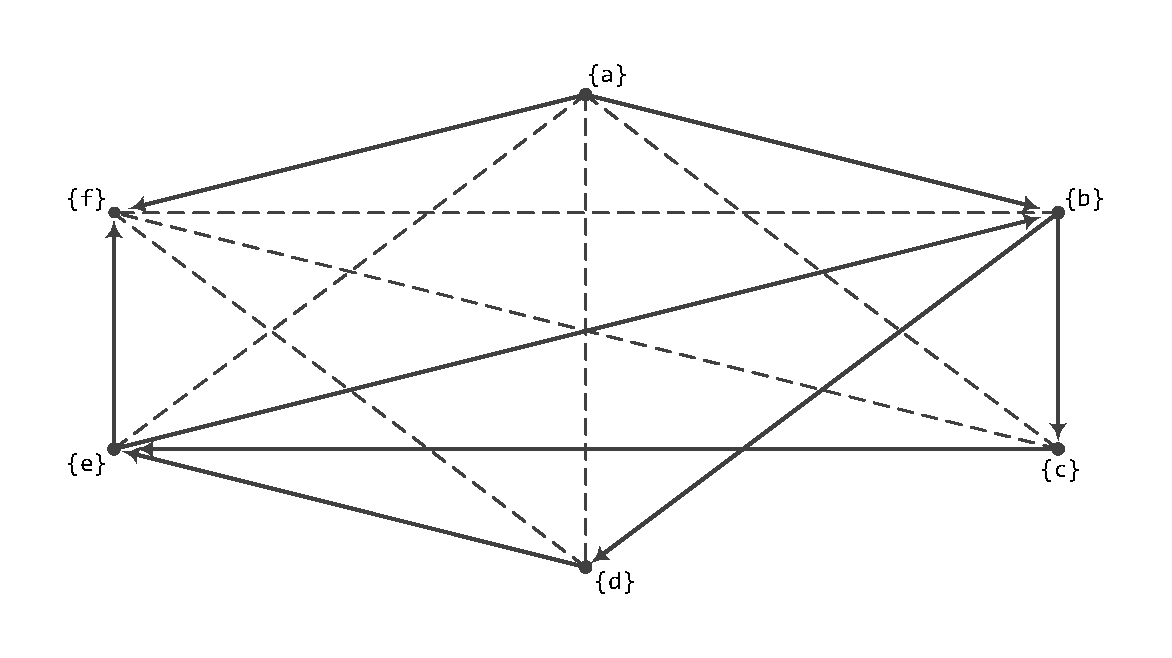
\includegraphics[width=0.8\textwidth]{pics/g_0.pdf}
\captionstyle{normal}\caption{Граф $G_0$ построенный для тестового журнала событий.}
\label{fig:g_0}
\end{figure}

После построения графа $G_0$ будем выполнять его последовательное расширение с помощью отдельных шагов.
На каждом шаге берется произвольное ребро $\overline{e} = \{X, Y\} \in \overrightarrow{E}$ и для него выполняются следующие действия.
В множество $N$ добавляется новый элемент $X \cup Y$.
Для каждого элемента $Z \in N$ такого, что $\{Z, X\} \in \overline{E}$, $\{Z, Y\} \in \overline{E}$ в множество неориентированных ребер $\overline{E}$ добавляется элемент $\{Z, X \cup Y\}$.
Для каждого элемента $Z \in N$ такого, что $(Z, X) \in \overrightarrow{E}$, $(Z, Y) \in \overrightarrow{E}$ в множество ориентированных ребер $\overrightarrow{E}$ добавляется элемент $(Z, X \cup Y)$, а в множество $\Xi$ добавляются элементы $((Z, X), (Z, X \cup Y))$ и $((Z, Y), (Z, X \cup Y))$.
Ребро $\overline{e}$ удаляется из множества $\overline{E}$.
Иллюстрация выполнения шага расширения графа $G$ представлена на рисунке~\ref{fig:step}.

\begin{figure}[h]
\setcaptionmargin{5mm}
\onelinecaptionsfalse % if the caption is multiline
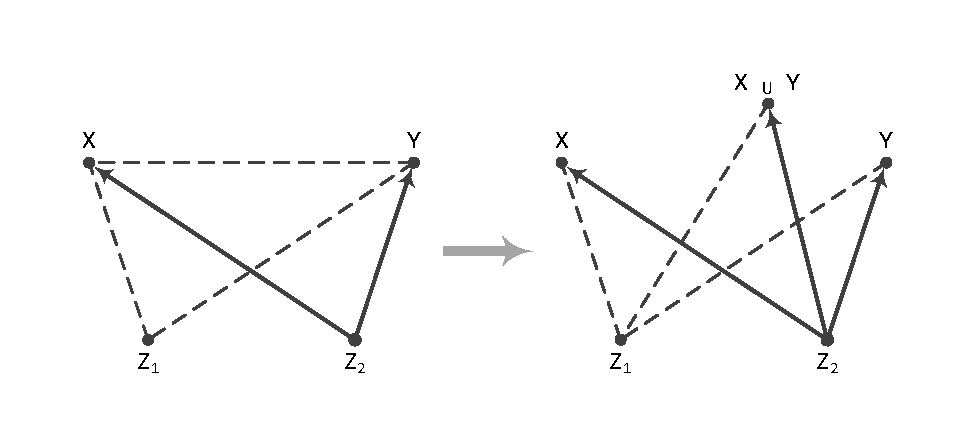
\includegraphics[width=0.8\textwidth]{pics/step.pdf}
\captionstyle{normal}\caption{Один шаг расширения графа отношений $G$.}
\label{fig:step}
\end{figure}

Описанные шаги по расширению графа $G$ выполняются до тех пор, пока множество $\overline{E}$ не станет пустым.
Стоит заметить, что количество элементов данного множества не обязано уменьшаться на каждом шаге расширения графа (например, на рисунке~\ref{fig:step} количество ребер из $\overline{E}$ не изменилось).
Однако, в том случае, если на каком-то шаге количество ребер в $\overline{E}$ не уменьшилось, то обязательно произошло разрушение полного графа, составленного из ребер из $\overline{E}$ (на рисунке~\ref{fig:step} разрушился треугольник $XYZ_1$), вместо которого может возникнуть полный граф только меньшего порядка.
Таким образом, через конечное количество шагов расширения множество $\overline{E}$ станет пустым и финальный граф $G$ будет сформирован.

\begin{figure}[h]
\setcaptionmargin{5mm}
\onelinecaptionsfalse % if the caption is multiline
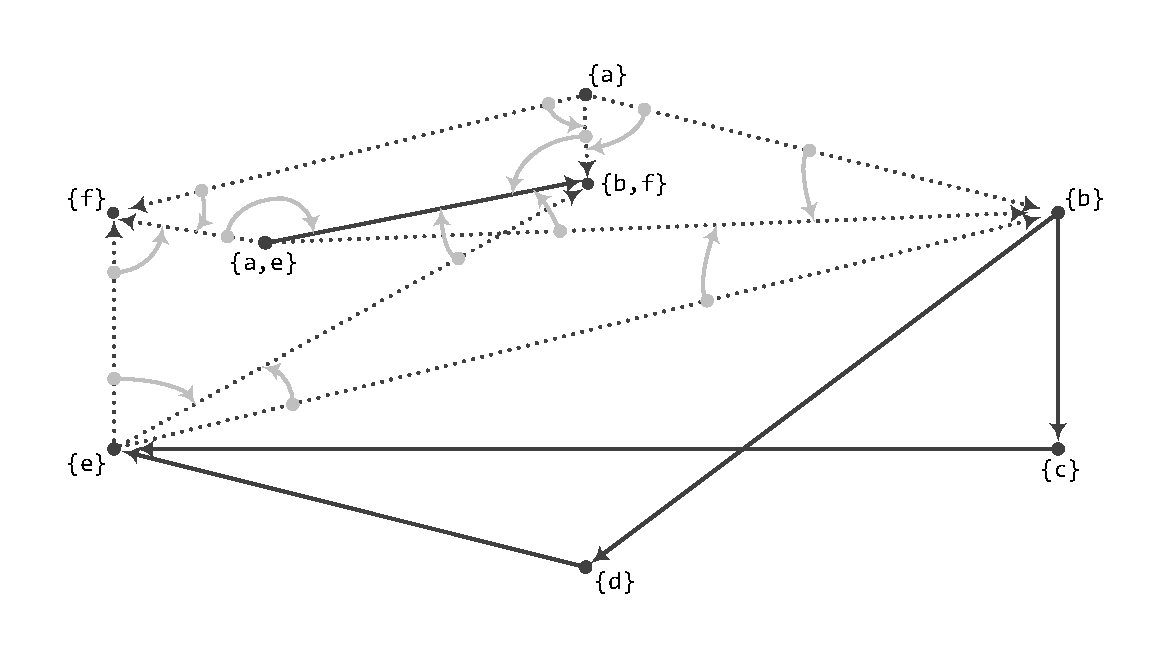
\includegraphics[width=0.8\textwidth]{pics/g.pdf}
\captionstyle{normal}\caption{Финальный вид графа отношений $G$.}
\label{fig:g}
\end{figure}

На рисунке~\ref{fig:g} приведен окончательный вид графа $G$ для рассматриваемого примера.
Элементы из множества $\Xi$ на данном рисунке показаны серыми дугами, а избыточные ребра из $\overrightarrow{E}$ изображены точечными линиями.
При описанном построении графа отношений $G$ не составляет труда обнаружить все избыточные ребра из $\overrightarrow{E}$.
Таким образом, искомое множество ребер из $\overrightarrow{E}$ изображено на рисунке сплошными черными стрелками, что совпадает с множеством из (\ref{eqn:p2}).

Недостатком алгоритма является то, что избыточные ребра нельзя удалять по ходу выполнения шагов расширения графа $G$, так как любое промежуточное ребро может участвовать при добавлении новых ребер.
Для устранения этого недостатка требуется проведение дополнительных исследований и усовершенствования данного алгоритма, что выходит за рамки данной статьи.

\section{Conclusion}

Conclusion.

\begin{acknowledgments}
The work has been done at the JSCC RAS as part of the state assignment for the topic ... The supercomputer MVS-10P, located at the JSCC RAS, was used for calculations during the research.
\end{acknowledgments}

\begin{thebibliography}{99}

\bibitem{Rettinger}
\refitem{article}
C. Rettinger, C. Godenschwager, S. Eibl, et al., {\it ``Fully Resolved Simulations of Dune Formation in Riverbeds"}, ISC High Performance , LNCS~{\bf 10266}, 3--21 (2017).

\end{thebibliography}

\end{document}
